\documentclass[12pt,a4paper,openany]{book}
\usepackage{lmodern}
\usepackage[svgnames]{xcolor} % Required to specify font color
\input{../LaTexTemplate/templates/couleurs.tex}

\usepackage{makeidx}
\usepackage[utf8]{inputenc} 
\usepackage{marvosym}
\usepackage[T1]{fontenc}
\usepackage[francais]{babel}
\usepackage[top=1.7cm, bottom=1.7cm, left=1.7cm, right=1.7cm]{geometry}
\usepackage{verbatim}
\usepackage[urlbordercolor={1 1 1}, linkbordercolor={1 1 1}, linkcolor=vert1, urlcolor=bleu, colorlinks=true]{hyperref}
\usepackage{tikz} %Vectoriel
\usepackage{listings}
\usepackage{fancyhdr}
\usepackage{multido}
\usepackage{amssymb}
\usepackage{float}
\usepackage[francais]{minitoc}
\usepackage[final]{pdfpages} 
\usepackage{graphicx} % Required for box manipulation
\usepackage{makeidx}

\newcommand{\titre}{FactDev -- V0.3}
\newcommand{\subtitle}{Manuel Utilisateur}
\newcommand{\auteur}{Équipe FACT}
\newcommand{\semestre}{~}
\newcommand{\annee}{2015}


\newcommand{\pole}{}
\newcommand{\sigle}{FACT}
\makeindex
\usepackage[totoc]{idxlayout}


\input{../LaTexTemplate/templates/listings.tex}
\input{../LaTexTemplate/templates/classroomsTemplates/l3/cours.tex}
\input{../LaTexTemplate/templates/remarquesExempleAttention.tex}
\input{../LaTexTemplate/templates/polices.tex}
\input{../LaTexTemplate/templates/affichageChapitre.tex}


\newcommand*{\plogo}{\fbox{$\mathcal{PL}$}} % Generic publisher logo
%----------------------------------------------------------------------------------------
%	TITLE PAGE
%----------------------------------------------------------------------------------------

\newcommand*{\rotrt}[1]{\rotatebox{90}{#1}} % Command to rotate right 90 degrees
\newcommand*{\rotlft}[1]{\rotatebox{-90}{#1}} % Command to rotate left 90 degrees

\newcommand*{\titleBC}{\begingroup % Create the command for including the title page in the document
\newlength{\drop} % Command for generating a specific amount of whitespace
\drop=0.1\textheight % Define the command as 10% of the total text height

\vspace*{-50px}
\rule{\textwidth}{0.4pt}\par % Thick horizontal line
\begin{tabular}{p{8cm}p{5cm}p{6cm}}
	\begin{minipage}{8cm}
		Équipe FACT\\
		\textit{Conception et développement d'applications}\\~\\
		\small
%		\Mobilefone~06~84~33~52~93\\
%		\Letter~\texttt{antoine.roquemaurel@gmail.com}\\
		\Mundus~\url{http://fact-team.github.io}
	\end{minipage} &
	& 

	\begin{minipage}{5cm}
		\begin{center}
			
\includegraphics[width=5cm]{logo.jpg}\\
			\tiny{Rédigé avec \LaTeX{}\\Version du \today}
		\end{center}
	\end{minipage}
\end{tabular}

\vspace{\drop} % Whitespace between the top lines and title
\centering % Center all text

\vspace{100px}
\def\CP{\textit{\Huge \titre}} % Title

\settowidth{\unitlength}{\CP} % Set the width of the curly brackets to the width of the title
{\color{LightGoldenrod}\resizebox*{\unitlength}{\baselineskip}{\rotrt{$\}$}}} \\[\baselineskip] % Print top curly bracket
\textcolor{Sienna}{\CP} \\[\baselineskip] % Print title
{\color{RosyBrown}\Large \subtitle} \\ % Tagline or further description
{\color{LightGoldenrod}\resizebox*{\unitlength}{\baselineskip}{\rotlft{$\}$}}} % Print bottom curly bracket

\vfill % Whitespace between the title and the author name


{
\normalsize \LARGE Université Toulouse III -- Paul Sabatier}\\ % Author name

\vfill % Whitespace between the author name and the publisher logo
\Large \today % Year published

\rule{\textwidth}{0.4pt}\par % Thick horizontal line

\endgroup}

%----------------------------------------------------------------------------------------
%	BLANK DOCUMENT
%----------------------------------------------------------------------------------------


\makeatother
\includeonly {
contents/intro,
%contents/1-1erLancement,
contents/2-ihm,
contents/3-donneesUtilisateur,
contents/4-clients,
contents/5-projets,
contents/6-devis,
contents/7-factures
}
\begin{document}
	\thispagestyle{empty} % Removes page numbers
	\titleBC 
	\dominitoc
	\setcounter{tocdepth}{1}
	\setcounter{secnumdepth}{3}
	\setcounter{minitocdepth}{1}
%	\maketitle
	
	
	\tableofcontents
	
	\begin{frame}{Les parties prenantes}
	\begin{itemize}
		\item \'Equipe FACT
			\begin{itemize}
				\item {Antoine de \bsc{Roquemaurel}
				\item Florent \bsc{Berbie}
				\item Cédric \bsc{Rohaut}
				\item Manantsoa Andriamihary \bsc{Razanajatovo}}
			\end{itemize}
			\vfill
		\item Encadrant
			\begin{itemize}
				\item Frédéric \bsc{Migeon}
			\end{itemize}
			\vfill
		\item Client
			\begin{itemize}
				\item Antoine de \bsc{Roquemaurel}
			\end{itemize}
			\vfill
	\end{itemize}
\end{frame}
\begin{frame}
	\tableofcontents	
\end{frame}


%	\chapter{1er lancement}
Au premier d\'emarrage du logiciel, une fen\^etre de configuration se lance.
Elle se compose d'une fen\^etre de << Bienvenue >>, d'une de configuration de la base de donn\'ees et d'une de saisi de vos informations personnelles.

\begin{figure}[H]
	\centering
	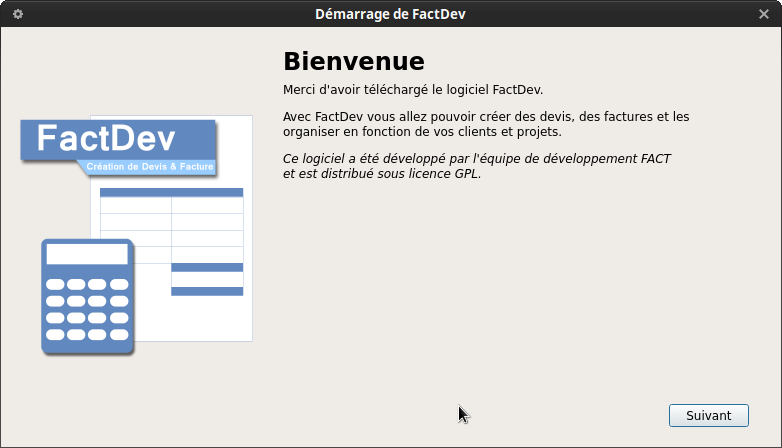
\includegraphics[width=12cm]{screens/lancement1.png}
	\caption{Premier lancement de FactDev}
	\label{fig:lancementFactDev}
\end{figure}

\section{Configuration de la base de donn\'ees}
Dans ces partie il faut choisir entre deux types de base de donn\'ees comme le montre les images ci-dessous.
\begin{figure}[H]
	\centering
	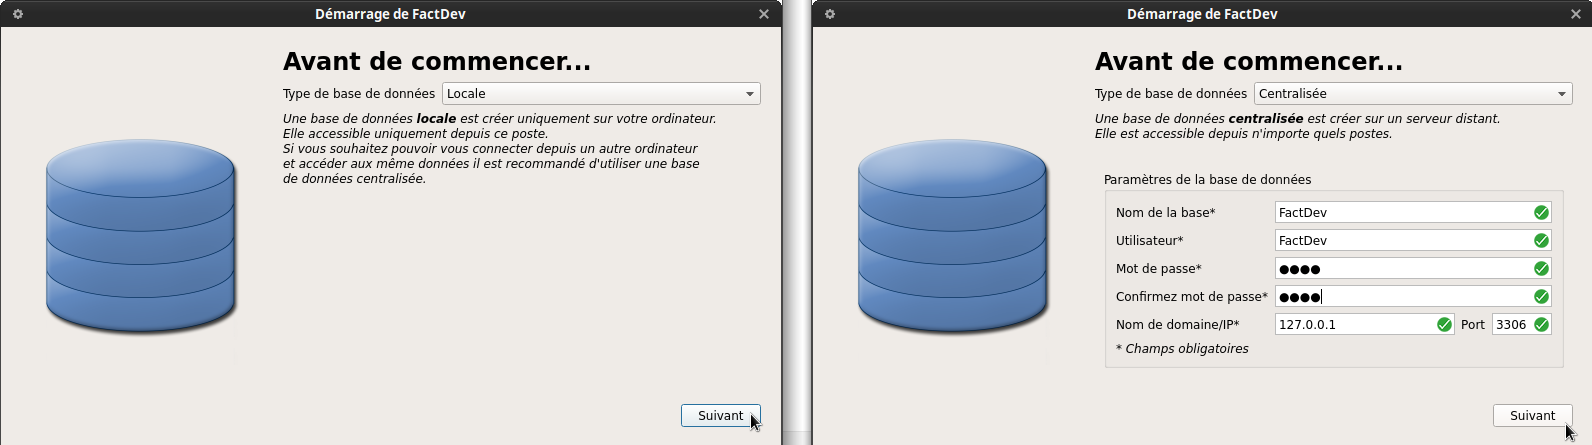
\includegraphics[width=15cm]{screens/lancement2.png}
	\caption{Configuration de la base de donn\'ees}
	\label{fig:configurationBaseDeDonnees}
\end{figure}
Le type de base de donn\'ees \textbf{locale} indique que les donn\'ees sont stock\'ees uniquement sur votre ordinateur. Vous aurez donc acc\`es \`a ces informations uniquement depuis ce poste. 

La base de donn\'ees \textbf{centralis\'ee} est cr\'eee sur un serveur distant. Cela signifie que, d\`es lors que l'on dispose d'une connexion internet, on peut acc\'eder aux donn\'ees du logiciel quelque soit l'ordinateur que l'on utilise. 
Dans ce dernier cas, des champs doivent \^etre renseign\'es: \\
\begin{description}
	\item[Nom de la base] (Obligatoire) Nom de la base de donn\'ees (FactDev par d\'efaut)
	\item[Utilisateur] (Obligatoire) Pseudo de l'utilisateur du logiciel (FactDev par d\'efaut)
	\item[Mot de passe] (Obligatoire) Mot de passe de l'utilisateur
	\item[Confirmez Mot de passe] (Obligatoire) V\'erifie que l'utilisateur a correctement saisi son mot de passe
	\item[Nom de domaine/IP] (Obligatoire) Nom de domaine du serveur distant ou son adresse IP (127.0.0.1 par d\'efaut)
	\item[Port] Num\'ero de port du serveur (3306 par d\'efaut)
\end{description} 

\section{Informations vous concernant}
La derni\`ere \'etape consiste \`a renseigner les informations de votre entreprise. 
\begin{figure}[H]
	\centering
	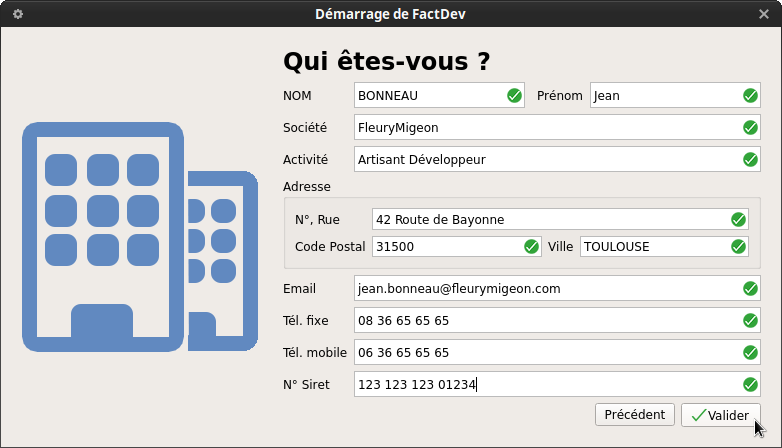
\includegraphics[width=12cm]{screens/lancement3.png}
	\caption{Renseignement des informations de l'entreprise}
	\label{fig:renseignementInformationsEntreprise}
\end{figure}
Les informations \`a renseigner sont:
\begin{description}
	\item[NOM] (Obligatoire) Votre NOM de famille
	\item[Pr\'enom] (Obligatoire) Votre pr\'enom
	\item[Soci\'et\'e] (Obligatoire) Le nom de votre soci\'et\'e
	\item[Activit\'e] Activit\'e de votre entreprise, slogan ou message qui la caract\'erise
	\item[Addresse] (Obligatoire) Adresse \`a laquelle se trouve votre entreprise
	\item[Email] (Obligatoire) Votre adresse e-mail professionnelle
	\item[T\'el\'ephone/Fax] Num\'ero de t\'el\'ephone (fixe ou mobile) et Fax. L'un des deux num\'eros de t\'el\'ephones doit obligatoirement \^etre renseign\'es. 
	\item[Num\'ero de Siret] (Obligatoire) Num\'ero de siret de votre soci\'et\'e (compos\'e de 14 chiffres)
\end{description} 



















	\chapter{Interface générale}
La fenêtre principale de l'application est divisé en cinq parties distinctes comme le montre la figure \ref{fig:ihm}. 

\begin{enumerate}
	\item \textbf{Client}. Vue globale de l'ensemble des clients et des informations qui leurs sont associés
	\item \textbf{Hiérarchie}. Actuellement composé uniquement de la liste des clients
	\item \textbf{Informations détaillées}. Affiche l'ensemble des informations d’un client sélectionné
	\item \textbf{Recherche}. Barre de recherche et filtres associés à la recherche
	\item \textbf{Barre de menu}. Bouton d’actions raccourcis
\end{enumerate}

\begin{figure}[H]
	\centering
	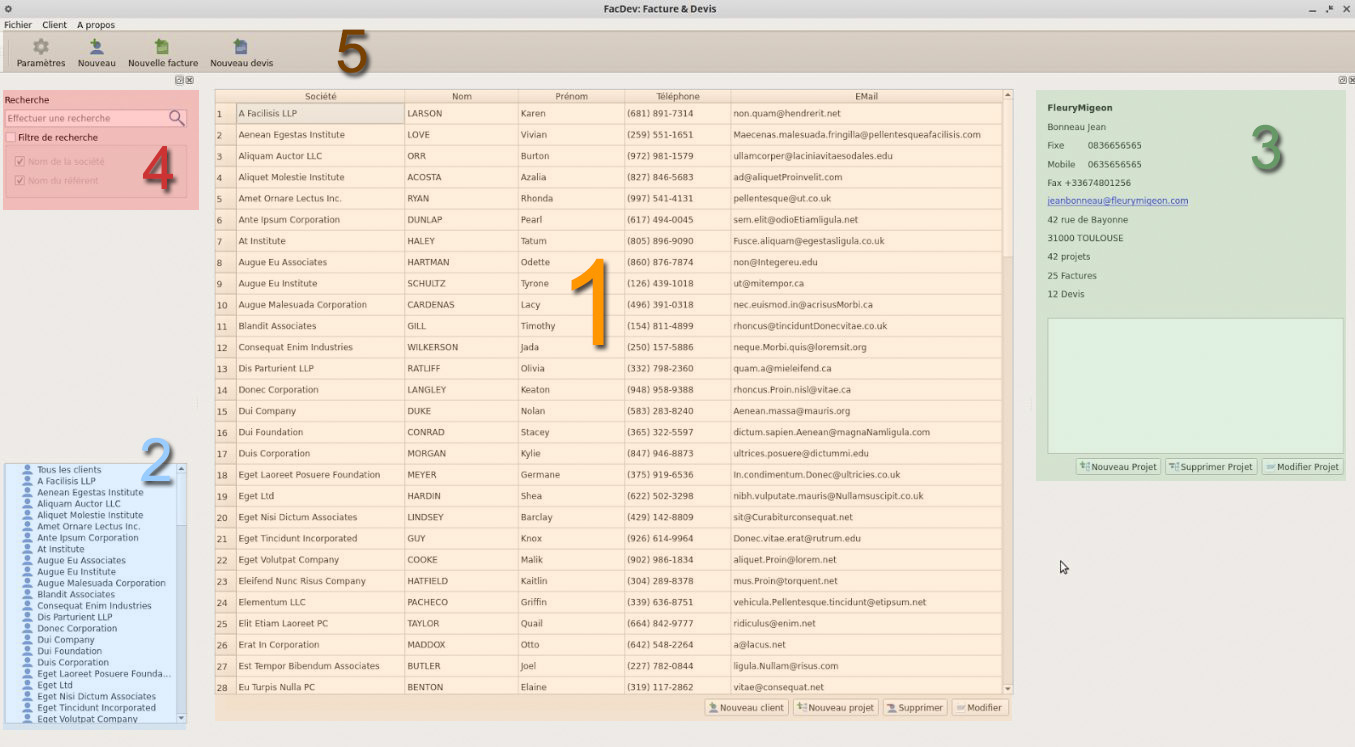
\includegraphics[width=10cm]{screens/ihm.jpg}
	\caption{Interface générale découpée en différentes parties}
	\label{fig:ihm}
\end{figure}

\section{Menus}
La plupart des fonctionnalités du logiciel sont disponibles via les menus situés en haut de l’application. 

\subsection{Fichier}
	\begin{description}
		\item[Paramètres] Permet d'afficher et de d’éditer l’utilisateur du logiciel.
		\item[Quitter] Quitte le logiciel
	\end{description}
\subsection{Client}
\begin{description}
	\item[Nouveau] Ajouter un nouveau client dans la base de données
	\item[Rechercher] Permet de rechercher un client dans la base de données
	\item[Nouvelle facture]  Ajouter une nouvelle facture à un projet d’un client dans la base de données
	\item[Nouveau devis] Ajouter un nouveau devis à un projet d’un client dans la base de données
\end{description}
\subsection{À propos}
\begin{description}
	\item[Qt] Informations sur le framework utilisé
	\item[Fact] Informations sur l'équipe de développement
	\item[FactDev]Informations sur le logiciel
	\item[Icons] Informations sur les icônes utilisées
\end{description}
\section{Barre d'outils}
La barre d’outils permet d’effectuer certaines actions de façon rapide, actions également disponibles via le menu.

\begin{description}
	\item[Paramètres] Permet d'afficher et de d’éditer l'utilisateur du logiciel. Disponible via le menu <<Fichier => Paramètres>>.
	\item[Nouveau] Ajouter un nouveau client dans la base de données. Disponible via le menu <<Client => Nouveau>>.
	\item[Nouvelle facture]  Ajouter une nouvelle facture à un projet d’un client dans la base de données. Disponible via le menu <<Client
		$\rightarrow$
		Nouvelle facture>>
	\item[Nouveau devis] Ajouter un nouveau devis à un projet d’un client dans la base de données. Disponible via le menu <<Client => Nouveau
		devis>>
\end{description}

\section{Panneau du client ou du référent}
Le panneau originellement situé à droite contient les informations du client ou du référent sélectionné, comme le montre la figure
\ref{fig:rightpanel}.

\begin{figure}[H]
	\centering
	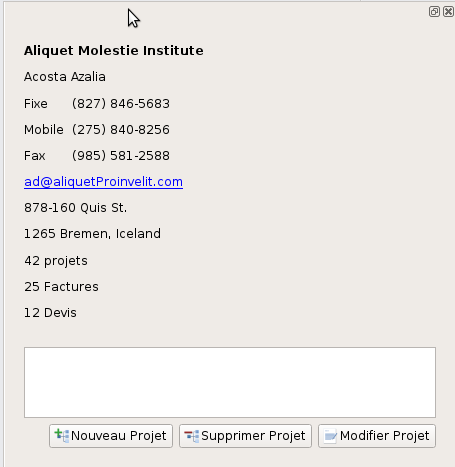
\includegraphics[width=10cm]{screens/dockDroite.png}
	\caption{Panneau du client ou du référent}
	\label{fig:rightpanel}
\end{figure}
% Il est possible d’ajouter un projet, d’en supprimer ou de modifier un projet du client via ce panneau. 
% TODO

\section{Panneau de recherche et sociétés}
Le panneau situé sur la gauche permet d’effectuer une recherche sur le nom de la société ou le nom du client ou du référent si la case
filtre de recherche est cochée et la recherche est faite selon le nom du référent. Cela permet de retrouver rapidement et facilement un
patient.

En dessous du champ de recherche sont affichés toutes les sociétés dans la base de données ainsi que les noms des clients ou référents
lorsque ceux-ci ne possèdent pas de société.





	\chapter{Les données utilisateur}
\section{Initialisation et modification des données de l'utilisateur}
L'initialisation des données de l'utilisateur se fait lors du premier démarrage du logiciel (cf.\ref{fig:renseignementInformationsEntreprise}).

Pour modifier ces informations, il suffit de cliquer sur le bouton \textbf{Paramètres}\index{Barre d'outils!Paramètres} de la barre d'outils \ref{fig:modifierUtilisateur} ou de passer par le menu <<Fichier $\rightarrow$ Paramètres>>. 

\begin{figure}[H]
	\centering
	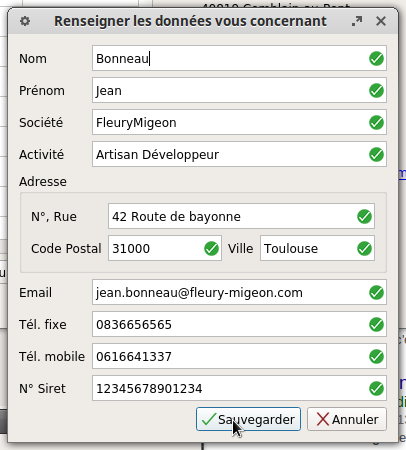
\includegraphics[height=8cm]{screens/modifierUtilisateur.png}
	\caption{Fenêtre de saisie des informations de l'utilisateur}
	\label{fig:modifierUtilisateur}
\end{figure}
	\chapter{Les clients}
Les clients sont le cœur de l'application, elle a donc besoin d'ajouter de nouveau clients pour pouvoir être utilisée. 
\begin{figure}[H]
	\centering
	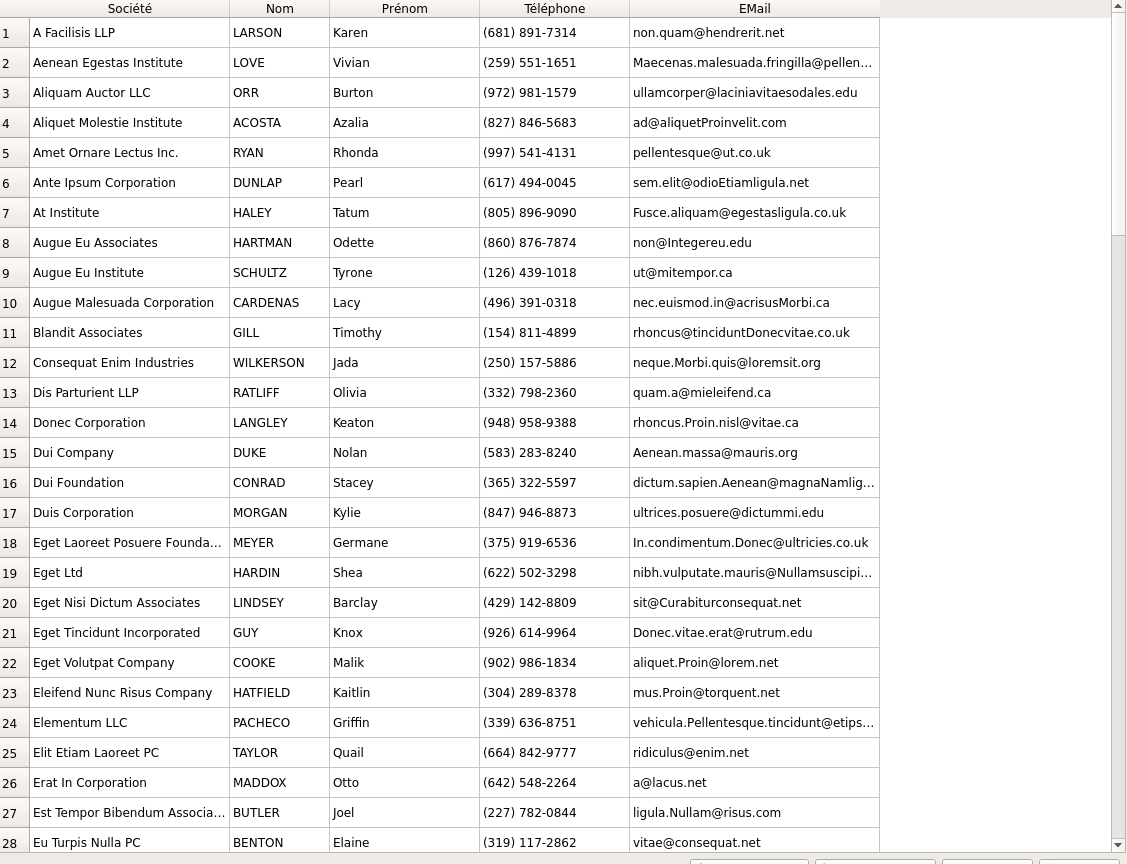
\includegraphics[width=12cm]{screens/clients.png}
	\caption{Gestion des clients}
\end{figure}

\section{Liste des clients\index{Client!Liste}}
La liste des clients, cf. figure 3.1, est accessible dès l’ouverture du logiciel. Celle-ci se trouve au centre du logiciel. 

La liste des clients contient uniquement les informations permettant de facilement les identifier à savoir, le nom de la société, le nom,
prénom, le numéro de téléphone et l’adresse e-mail. La sélection dans le tableau de l’un des clients permet, via le panneau du client,
d’obtenir les informations détaillées sur celui-ci. 

\section{Ajout d'un client\index{Client!Ajouter}}
L'ajout d’un patient peut se faire soit via le menu <<Client $\rightarrow$ Nouveau Client>>, via la barre d'outils ou encore via le bouton situé sous la
liste. 
\begin{figure}[H]
	\centering
	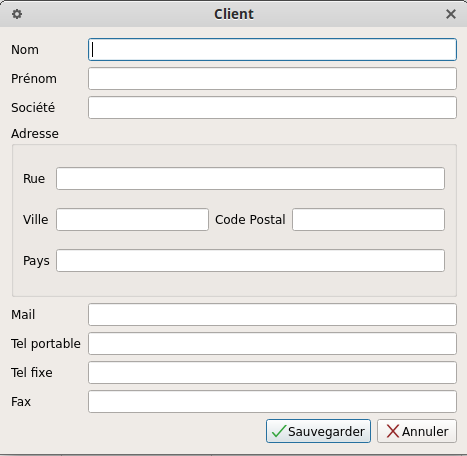
\includegraphics[width=7cm]{screens/ajouterClient.png}
	\caption{Ajouter un client}
\end{figure}

\section{Édition d'un client\index{Client!Éditer}}
L’édition d’un client a pour but de corriger d’éventuels erreurs sur les informations d’un client. Pour ce faire, il suffit de sélectionner
un client dans le tableau et de cliquer sur le bouton <<Modifier>> situé sous la liste des clients ou, via le menu contextuel, lors d’un clic
droit sur le client dans le tableau. 
 La fenêtre est similaire à celle lors d’un ajout de client, seul diffère les champs qui sont déjà pré-remplis. 


	\chapter{Les projets}
La gestion des clients associe à chacun d'eux un ou plusieurs projets : il est donc nécessaire de visualiser la liste des projets pour chacun des clients. 
\begin{figure}[H]
	\centering
	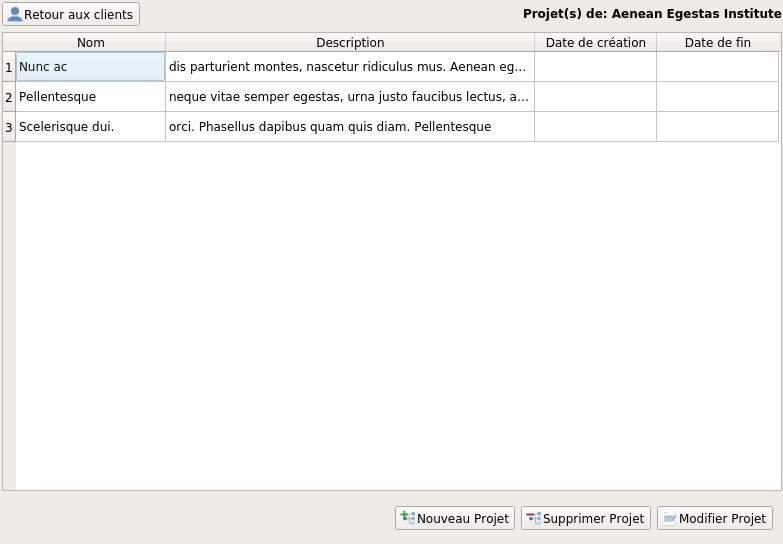
\includegraphics[width=12cm]{screens/projets.png}
	\caption{Gestion des projets d'un client}
\end{figure}

\section{Liste des projets\index{Projet!Liste}}
La liste des projets d'un client se trouve soit dans l'arborescence de la vue hiérarchique\index{Panneau!Hiérarchie} en déroulant la liste des projets d'un client soit en faisant un double clic sur l'un des clients de la liste du panneau centrale. Dans les deux cas, cela modifie le panneau principal qui contient maintenant la liste des projets pour le client comme le montre la figure ci-dessous.
\begin{figure}[H]
	\centering
	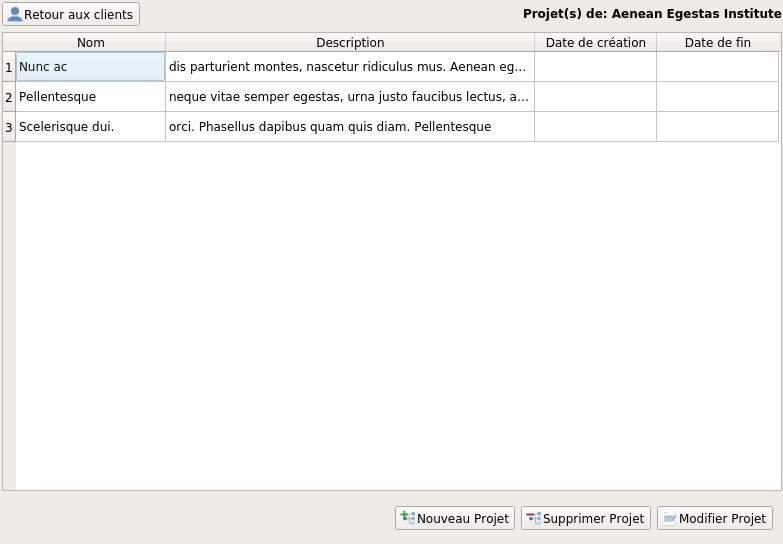
\includegraphics[width=10cm]{screens/projets.png}
	\caption{Liste des projets}
\end{figure}
La liste des projets contient les informations de chacun des projets c'est-à-dire un nom de projet, une description, les dates de début et de fin de projet. 

\section{Ajout d'un projet\index{Projet!Ajouter}}
L'ajout d’un projet peut se faire via le bouton <<Nouveau projet>> en bas du panneau principal.
Cependant, selon que le panneau central soit la liste des clients ou celle des projets, l'interface diffère. En effet, dans le premier cas il faut associer un projet à un client. 
C'est pour cela que la fenêtre propose un tableau avec la liste des clients afin de sélectionner celui auquel on veut associer un projet. 
Une barre de recherche permettant de retrouver facilement un client dans la liste est présente dans l'interface. Pour qu'un projet puisse être ajouté il devra obligatoirement être associé à un client et avoir un nom. 
Il est également possible d'ajouter une courte description et de mentionner le coût horaire ou journalier du projet. 
\begin{figure}[H]
	\centering
	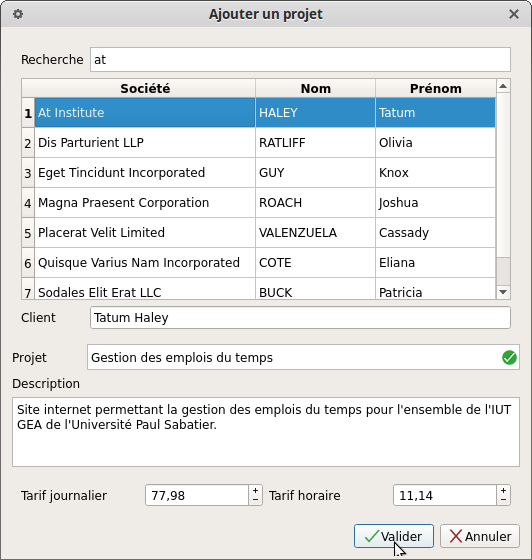
\includegraphics[width=7cm]{screens/ajouterProjet.png}
	\caption{Ajouter un projet}
\end{figure}
Dans le cas où le panneau central contient la liste des projets, cela signifie que ces projets sont ceux d'un client. C'est pourquoi, lorsqu'on clic sur le bouton <<Nouveau projet>>, celui-ci est automatiquement affecté au client courant. 
\begin{figure}[H]
	\centering
	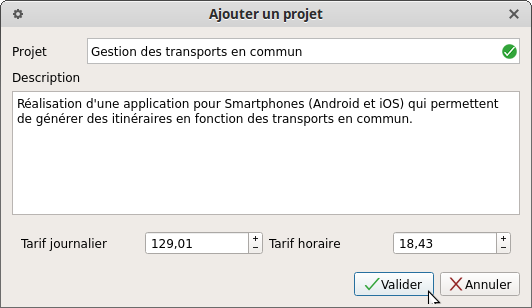
\includegraphics[width=7cm]{screens/ajouterProjetClient.png}
	\caption{Ajouter un nouveau projet à un client}
\end{figure}

\section{Édition d'un projet\index{Projet!Éditer}}
L’édition d’un projet a pour but de corriger d’éventuelles erreurs sur les informations d’un projet. Pour ce faire, il suffit de sélectionner un projet dans le tableau et de cliquer sur le bouton <<Modifier>> situé sous la liste des projets. 
La fenêtre est similaire à celle lors de l'ajout d'un projet à un client, seul diffère les champs qui sont pré-remplis. 
\begin{figure}[H]
	\centering
	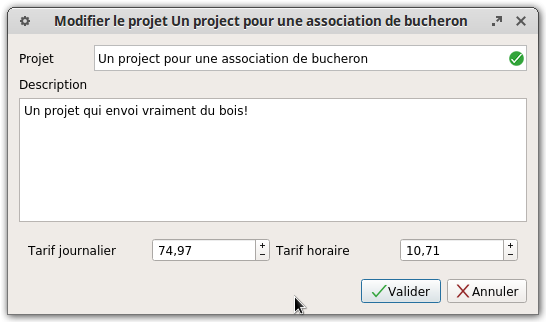
\includegraphics[width=7cm]{screens/editerProjet.png}
	\caption{Éditer un projet}
\end{figure}
	\chapter{Les devis\index{Devis}}
Les devis représente l'une des fonctionnalité principale de l'application. Il est possible de créer plusieurs devis pour un seul projet d'un client. 
\section{Les des devis\index{Devis!Liste}}

\section{Ajouter un devis\index{Devis!Ajouter}}

\section{Les Prestations\index{Devis!Prestation}}

	\chapter{Les factures}
Les factures sont tout comme les devis une des fonctionnalités les plus importantes de l'application. De propriétés semblable, il est aussi possible de créer plusieurs factures pour un projet.
\section{Liste des factures\index{Facture!Liste}}
Pour afficher les factures d'un projet il faut comme pour les devis, à partir du panneau contenant la liste des projets d'un client, faire un double clic sur le projet en question. La liste affichée contient les factures et les devis du projet sélectionné auparavant.

\section{Ajouter une facture\index{Facture!Ajouter}}
Pour ajouter une facture, il est nécessaire de sélectionner un client dans le panneau central (si l'on est dans la liste des projets ou des factures, la nouvelle facture sera automatiquement ajoutée à ce client). Une fois le client selectionné on crée une nouvelle facture en cliquant sur le bouton << Nouvelle facture >> de la barre d'outils ou via le menu << Client $\rightarrow$ Nouvelle facture >>. 
\begin{figure}[H]
	\centering
	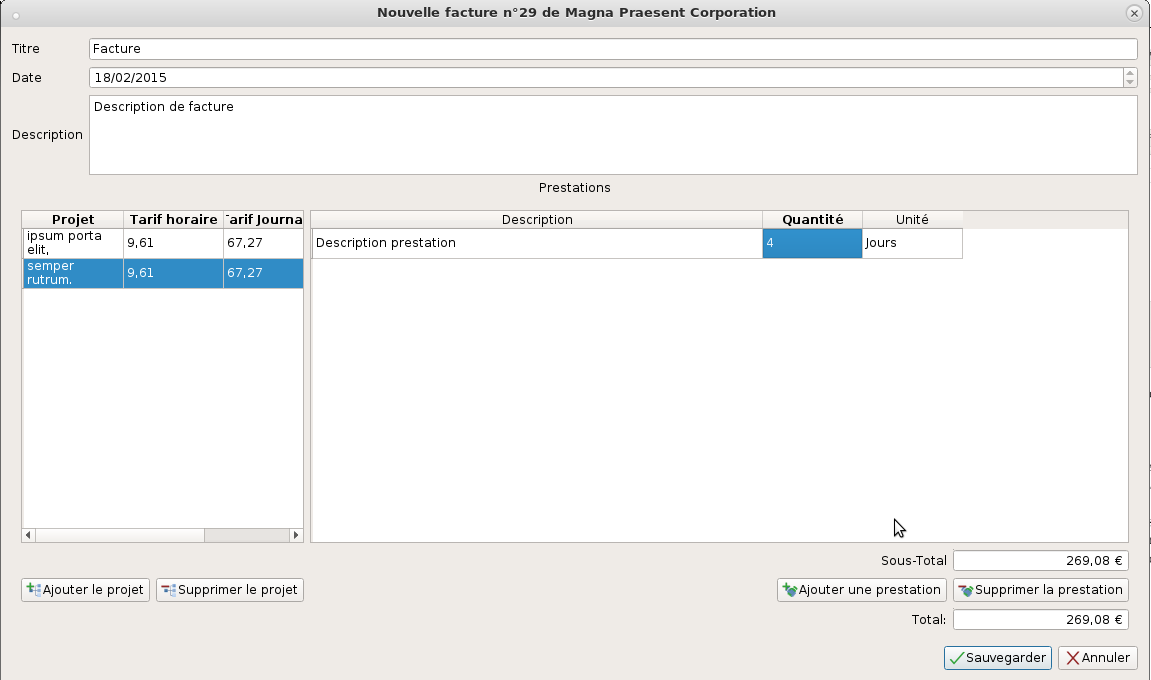
\includegraphics[width=15cm]{screens/creerFacture.png}
	\caption{Créer une nouvelle facture à un projet client}
\end{figure}
Une facture possède un titre à afficher, une date (celle du jour de création du projet), une description et deux tableaux exactement comme lors de la création ou l'édition d'un devis. Le fonctionnement est le même que pour un devis.
\section{Les Prestations\index{Facture!Prestation}}
Les prestations ont exactement le même comportement que lorsqu'on fait une création ou une édition d'un devis.
	\appendix
	\listoffigures
	\printindex

\end{document}
